% Options for packages loaded elsewhere
\PassOptionsToPackage{unicode}{hyperref}
\PassOptionsToPackage{hyphens}{url}
%
\documentclass[
]{article}
\usepackage{amsmath,amssymb}
\usepackage{iftex}
\ifPDFTeX
  \usepackage[T1]{fontenc}
  \usepackage[utf8]{inputenc}
  \usepackage{textcomp} % provide euro and other symbols
\else % if luatex or xetex
  \usepackage{unicode-math} % this also loads fontspec
  \defaultfontfeatures{Scale=MatchLowercase}
  \defaultfontfeatures[\rmfamily]{Ligatures=TeX,Scale=1}
\fi
\usepackage{lmodern}
\ifPDFTeX\else
  % xetex/luatex font selection
\fi
% Use upquote if available, for straight quotes in verbatim environments
\IfFileExists{upquote.sty}{\usepackage{upquote}}{}
\IfFileExists{microtype.sty}{% use microtype if available
  \usepackage[]{microtype}
  \UseMicrotypeSet[protrusion]{basicmath} % disable protrusion for tt fonts
}{}
\makeatletter
\@ifundefined{KOMAClassName}{% if non-KOMA class
  \IfFileExists{parskip.sty}{%
    \usepackage{parskip}
  }{% else
    \setlength{\parindent}{0pt}
    \setlength{\parskip}{6pt plus 2pt minus 1pt}}
}{% if KOMA class
  \KOMAoptions{parskip=half}}
\makeatother
\usepackage{xcolor}
\usepackage[margin=1in]{geometry}
\usepackage{listings}
\newcommand{\passthrough}[1]{#1}
\lstset{defaultdialect=[5.3]Lua}
\lstset{defaultdialect=[x86masm]Assembler}
\usepackage{graphicx}
\makeatletter
\def\maxwidth{\ifdim\Gin@nat@width>\linewidth\linewidth\else\Gin@nat@width\fi}
\def\maxheight{\ifdim\Gin@nat@height>\textheight\textheight\else\Gin@nat@height\fi}
\makeatother
% Scale images if necessary, so that they will not overflow the page
% margins by default, and it is still possible to overwrite the defaults
% using explicit options in \includegraphics[width, height, ...]{}
\setkeys{Gin}{width=\maxwidth,height=\maxheight,keepaspectratio}
% Set default figure placement to htbp
\makeatletter
\def\fps@figure{htbp}
\makeatother
\setlength{\emergencystretch}{3em} % prevent overfull lines
\providecommand{\tightlist}{%
  \setlength{\itemsep}{0pt}\setlength{\parskip}{0pt}}
\setcounter{secnumdepth}{-\maxdimen} % remove section numbering

\usepackage{listings}
\usepackage{color} 
\usepackage[dvipsnames]{xcolor}

\lstset{
  language=R,                     % the language of the code
  basicstyle=\footnotesize\ttfamily, % the size of the fonts that are used for the code
  numbers=left,                   % where to put the line-numbers
  numberstyle=\footnotesize\color{Black},  % the style that is used for the line-numbers
  stepnumber=1,                   % the step between two line-numbers. If it is 1, each line
  numbersep=5pt,                  % how far the line-numbers are from the code
  backgroundcolor=\color{white},  % choose the background color. You must add \usepackage{color}
  showspaces=false,               % show spaces adding particular underscores
  showstringspaces=false,         % underline spaces within strings
  showtabs=false,                 % show tabs within strings adding particular underscores
  rulecolor=\color{black},        % if not set, the frame-color may be changed on line-breaks within not-black text (e.g. commens (green here))
  tabsize=2,                      % sets default tabsize to 2 spaces
  captionpos=b,                   % sets the caption-position to bottom
  breaklines=true,                % sets automatic line breaking
  breakatwhitespace=false,        % sets if automatic breaks should only happen at whitespace
  keywordstyle=\color{RoyalBlue},      % keyword style
  commentstyle=\color{darkgray},   % comment style
  stringstyle=\color{ForestGreen},
  breaklines=true,
  aboveskip=\baselineskip,   % Space above the code block
  belowskip=\baselineskip
}

\ifLuaTeX
  \usepackage{selnolig}  % disable illegal ligatures
\fi
\usepackage{bookmark}
\IfFileExists{xurl.sty}{\usepackage{xurl}}{} % add URL line breaks if available
\urlstyle{same}
\hypersetup{
  pdftitle={The role of oceanographic connectivity in population differentiation},
  pdfauthor={-----},
  hidelinks,
  pdfcreator={LaTeX via pandoc}}

\title{The role of oceanographic connectivity in population
differentiation}
\usepackage{etoolbox}
\makeatletter
\providecommand{\subtitle}[1]{% add subtitle to \maketitle
  \apptocmd{\@title}{\par {\large #1 \par}}{}{}
}
\makeatother
\subtitle{coastalNet Package}
\author{-----}
\date{2024-03-23}

\begin{document}
\maketitle

Oceanographic connectivity driven by the direction and intensity of
ocean currents can shape the distribution of intraspecific biodiversity
(i.e., the genetic differentiaiton levels).

This code example explores how oceanographic connectivity influences
genetic differentiation in a kelp species (Laminaria ochroleuca). It
starts by loading data on kelp sampling locations and their genetic
differences. Then, it retrieves oceanographic connectivity information
from a database for the study region. The code calculates pairwise
connectivity probabilities between sampling sites, considering
multigeneration stepping-stone connections. Next, it builds a
statistical model to see if higher connectivity is linked to greater
genetic differentiation among kelp populations. The code visualizes this
relationship with a scatterplot and creates a map to show the
connections between sampling sites, with thicker lines indicating
stronger connectivity.

By combining oceanographic connectivity information derived from
coastalNet package withh empirical genetic data, this script
demonstrates that intraspecific biodiversity can be highly structured by
connectivity driven by oceanographic transport and barriers.

Here's a summary of the key steps and functions encapsulated in the
code:

\subsubsection{Environment Preparation and Package
Loading}\label{environment-preparation-and-package-loading}

Cleans the R environment and forces garbage collection to ensure a clean
workspace. Loads necessary R packages for the analysis, which include
coastalNet package.

\begin{lstlisting}[language=R]
# Clean environment and load packages
rm(list = ls())
gc(reset=TRUE)

library(coastalNet)

library(ggplot2)
library(sf)
library(lme4)
library(rnaturalearth)
library(viridis)
sf_use_s2(FALSE)
\end{lstlisting}

\subsubsection{Data Loading}\label{data-loading}

Imports two CSV files from a GitHub repository: laminariaRecords:
Contains geographical coordinates (longitude and latitude, WGS84) of
sampled sites for Laminaria ochroleuca. laminariaPopDifferentiation:
Contains pairwise genetic differentiation estimates between the sampled
sites.

\begin{lstlisting}[language=R]

# Load data.frame containing coordinates (as longitude and longitude, WGS84) of sites sampled for the marine species Laminaria ochroleuca.
laminariaRecords <- read.csv("https://raw.githubusercontent.com/jorgeassis/coastalNet/main/vignettes/data/Laminaria-ochroleuca-Coords.csv", sep=";", header = TRUE)

# Load data.frame containing pairwise genetic differentiation estimates between coordinate sites
laminariaPopDifferentiation <- read.csv("https://raw.githubusercontent.com/jorgeassis/coastalNet/main/vignettes/data/Laminaria-ochroleuca-JostD.csv", sep=";", header = FALSE)
\end{lstlisting}

\subsubsection{Connectivity Analysis}\label{connectivity-analysis}

Initializes a local database for storing analysis results (if not
already present). Determines hexagon IDs defining the study region based
on the extent of the sampled sites, with a specified buffer. Calculates
connectivity events within the study region for a specified period (120
days), considering all years, months, and days. Obtains pairwise
connectivity estimates between the sampled sites using a forward
connectivity type, considering the probability of connectivity and
allowing for stepping-stone connections.

\begin{lstlisting}[language=R]
# Load database
getDataBase(myFolder="Database", overwrite=FALSE)

# Get hexagon IDs that define the study region
hexagonIDRegion <- getHexagonID(obj=laminariaRecords, level="extent", buffer=5, print=TRUE)
\end{lstlisting}

\begin{figure}
\centering
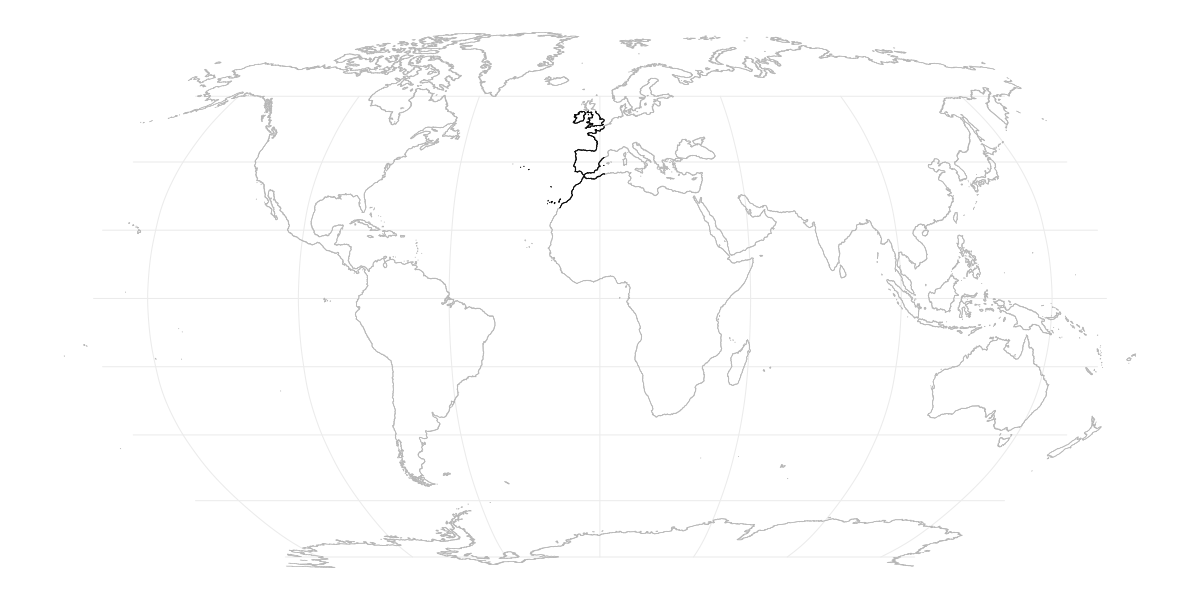
\includegraphics{../img/Example1_img_1.png}
\caption{Hexagon IDs (in black) defining the study region}
\end{figure}

\begin{lstlisting}[language=R]
# Get connectivity events for the study region (all years, all months, all days, 120 days period)
connectivityEvents <- getConnectivityEvents(hexagonID=hexagonIDRegion, period=120 )

# Get hexagon IDs of the sampling sites
hexagonIDSites <- getHexagonID(obj=laminariaRecords, level="site", buffer=0, print=FALSE)

# Get pairwise connectivity estimates between coordinate sites
pairwiseConnectivity <- getPairwiseConnectivity(connectivityEvents, hexagonIDFrom=hexagonIDSites, connType="Forward", value="Probability", steppingStone=TRUE)
\end{lstlisting}

\subsubsection{Data Preparation for
Modeling}\label{data-preparation-for-modeling}

Constructs a data frame to match pairs of oceanographic connectivity
with pairs of population differentiation for all site pairs, excluding
self-comparisons. Cleans the data frame by removing zero connectivity
values and missing data, and applies a negative log transformation to
the connectivity values.

\begin{lstlisting}[language=R]
# Produce and data.frame matching pairs of oceanographic connectivity and pairs of population differentiation 
modelDataFrame <- data.frame()
for( from in 1:nrow(laminariaRecords)) {
  for( to in 1:nrow(laminariaRecords)) {
    if( from == to ) { next }
    modelDataFrame <- rbind(modelDataFrame,data.frame(from = from, to = to, connectivity = mean(pairwiseConnectivity$connectivityMatrix[from,to], pairwiseConnectivity$connectivityMatrix[to,from], na.rm=T), differentiation = laminariaPopDifferentiation[from,to]))
  }
}

# Remove zero connectivity values, missing values and Log-transform connectivity
modelDataFrame <- modelDataFrame[modelDataFrame$connectivity != 0 ,]
modelDataFrame <- modelDataFrame[complete.cases(modelDataFrame),]
modelDataFrame$connectivity <- log(modelDataFrame$connectivity)
\end{lstlisting}

\subsubsection{Statistical Modeling}\label{statistical-modeling}

Fits a linear model to examine the relationship between oceanographic
connectivity and population differentiation. Calculates the adjusted
R-squared value and Pearson's correlation coefficient to access the
relationship.

\begin{lstlisting}[language=R]
# Model oceanographic connectivity to population differentiation
model <- lm(connectivity ~ differentiation, data = modelDataFrame)
r2 <- summary(model)$adj.r.squared
Pearson <- cor(modelDataFrame$connectivity, modelDataFrame$differentiation)
\end{lstlisting}

\subsubsection{Visualization}\label{visualization}

Produces two plots: A scatter plot showing Oceanographic connectivity
{[} log(probability) {]} versus Population genetic differentiation
(Fst), including a regression line, and displaying the adjusted
R-squared and Pearson's correlation coefficient. A map visualizing the
stepping-stone oceanographic connectivity between populations,
overlaying the sampled sites on a world map and depicting connectivity
paths.

\begin{lstlisting}[language=R]
plot1 <- ggplot() + 
  geom_point(data = modelDataFrame, aes(x=connectivity, y=differentiation), color="#000000", fill="#000000", size=2 ) + 
  geom_point(data = modelDataFrame, aes(x=connectivity, y=differentiation), color="white", fill="white", size=1 ) + 
  geom_smooth(data = modelDataFrame, method=lm, aes(x=connectivity, y=differentiation), linetype = "dashed", fill="#c5593c", col='black', size=0.5, alpha = 0.5) + 
  xlab(paste0("Oceanographic connectivity [ log(probability) ]")) + ylab("Population genetic differentiation (Fst)") +
  theme_minimal() + 
  theme( panel.grid.major = element_blank() ,
         text = element_text(size=12) ,
         axis.title.y = element_text(margin = margin(t = 0, r = 18, b = 0, l = 0)) ,
         axis.title.x = element_text(margin = margin(t = 18, r = 0, b = 0, l = 0)) ,
         legend.title = element_blank()) +
         annotate("label", alpha = 0.5, label.padding=unit(0.5, "lines"), x = -77, y = 0.2, hjust=0,vjust=1 , label = paste0("Adjusted R2: ", format(round(r2, 3), nsmall = 3),"\nPearson's Corr.: ",format(round(Pearson, 3), nsmall = 3)))

plot1
\end{lstlisting}

\begin{figure}
\centering
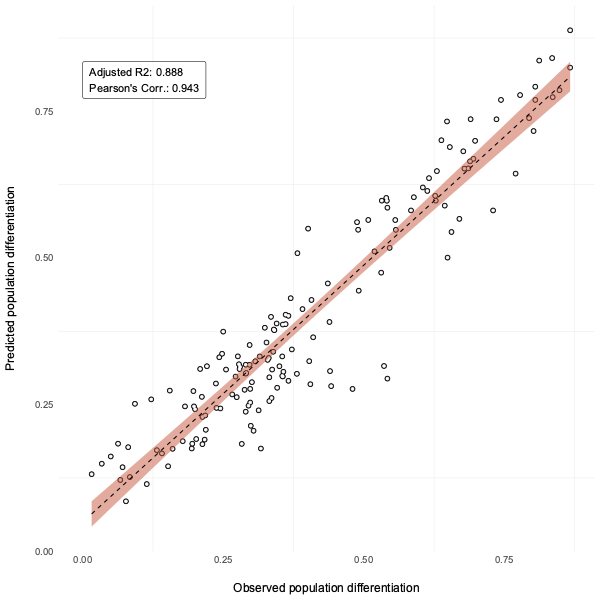
\includegraphics[width=0.75\textwidth,height=\textheight]{../img/Example1_img_2.png}
\caption{Role of oceanographic connectivity to population
differentiation}
\end{figure}

\begin{lstlisting}[language=R]
# Map oceanographic connectivity between populations
mappedConnectivity <- mapConnectivity(connectivityPairs=pairwiseConnectivity$connectivityPairs)

# Load the worldmap and crop to the atudy region
worldMap <- ne_countries(scale = "medium", returnclass = "sf")
worldMap <- st_crop(worldMap,c(xmin=min(laminariaRecords[,1])-5,xmax=max(laminariaRecords[,1])+5,ymin=min(laminariaRecords[,2])-2.5,ymax=max(laminariaRecords[,2])+2.5))

# Get hexagon IDs that retrieved oceanographic connectivity estimates
hexagonIDConnected <- unique(c(mappedConnectivity$mappingData$FromHexagon,mappedConnectivity$mappingData$FromHexagon))

# Get a data.frame of the location of hexagons that retrieved oceanographic connectivity estimates
data("hexagonCells")
hexagonCellsConnected <- hexagonCells[hexagonCells$ID %in% hexagonIDConnected,1]
hexagonCellsConnected <- st_coordinates(st_centroid(hexagonCellsConnected))

# Make a plot of the oceanographic connectivity between populations
plot2 <- ggplot() + 
  geom_sf(data = worldMap , fill="#CDCDCD", colour = "#9E9E9E" , size=0.25) +
  geom_point(data = hexagonCellsConnected, aes(x = X, y = Y), colour = "#000000",size=2.5) +
  geom_point(data = hexagonCellsConnected, aes(x = X, y = Y), colour = "#FFFFFF",size=1.25) +
  geom_sf(data = mappedConnectivity$lineConnections , linewidth = 0.35 , aes(colour = Value), alpha=0.75) +
  scale_color_gradientn(colours=rev(magma(6)),na.value = NA, trans = "log") +
  theme_minimal() + theme(axis.title.x=element_blank(),
                          axis.ticks.x=element_blank(),
                          axis.title.y=element_blank(),
                          axis.ticks.y=element_blank(), legend.position = "none") +
  coord_sf()

plot2
\end{lstlisting}

\begin{figure}
\centering
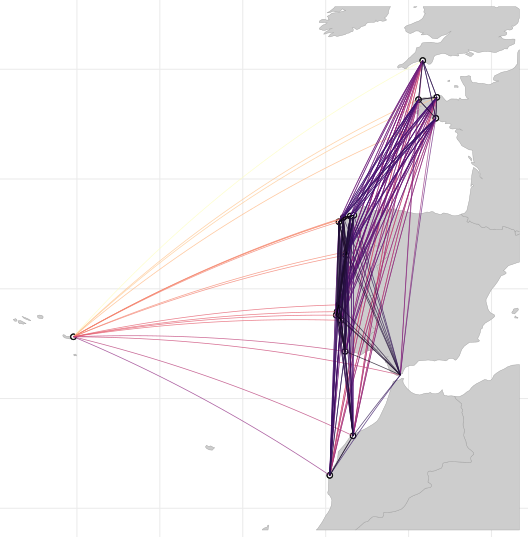
\includegraphics[width=0.75\textwidth,height=\textheight]{../img/Example1_img_3.png}
\caption{Stepping-stone oceanographic connectivity between populations}
\end{figure}

\end{document}
